\section{Objetivos}

\begin{frame}
	\frametitle{Objetivos}
	\begin{itemize}
		\item Introduzir o conceito de \textbf{algoritmo}
		\item Apresentar abordagens de representações de algoritmos
		\item Desenvolver algoritmos
	\end{itemize}
\end{frame}



\section{Algoritmo}

\begin{frame}
	\frametitle{Algoritmo}
	\begin{block}{\textbf{Conceito de Algoritmo}}
		\begin{itemize}
			\item ``Algoritmo é uma sequência de passos que visa atingir um objetivo bem definido.'' (FORBELLONE, 1999)
			\item ``Algoritmo é a descrição de uma sequência de passos que deve ser seguida para a realização de uma tarefa.'' (ASCENCIO, 1999)
		\end{itemize}
	\end{block}
	
	\textbf{Exemplos}:\\
	- Receita de bolo\\
	- Trocar o pneu de um carro\\[2ex]

	\textbf{Padrão}:\\
	- Determina um padrão de comportamento a ser seguido para alcançar um objetivo.
\end{frame}


\begin{frame}
	\frametitle{Algoritmo no dia-a-dia}
	\begin{itemize}
		\item Executamos vários algoritmos no dia-a-dia: 
		\begin{itemize}
			\item \textbf{Fazer um sanduíche}
			\item \textbf{Dividir a conta da lanchonete}
			\item \textbf{Trocar uma lâmpada}
			\item \textbf{Ir para a escola}
			\item \textbf{Sacar dinheiro}
			\item \textbf{Calçar sapatos}
		\end{itemize}
	\end{itemize}
\end{frame}


\begin{frame}
	\frametitle{Algoritmo no dia-a-dia}
	\begin{itemize}
		\item Problema: \textbf{Fazer um sanduíche}
		\item Entradas: pão, maionese, alface e hambúrguer
		\item Processamento: adicionar os ingredientes dentro do pão
		\item Saída: um sanduíche
		\item Algoritmo:
		\begin{itemize}
			\item Passo 1 - Pegar o pão
			\item Passo 2 - Cortar o pão
			\item Passo 3 - Pegar a maionese
			\item Passo 4 - Passar a maionese no pão
			\item Passo 5 - Colocar o alface e tomate no pão
			\item Passo 6 - Pegar o hambúrguer
			\item Passo 7 - Fritar o hambúrguer
			\item Passo 8 - Colocar o hambúrguer no pão
			\item Passo 9 - Colocar o queijo no pão
		\end{itemize}
	\end{itemize}
\end{frame}



\begin{frame}
	\frametitle{Algoritmo no dia-a-dia}
	\begin{itemize}
		\item Problema: \textbf{Fazer um sanduíche}
		\item Algoritmo:
		\begin{itemize}
			\item<1-> Passo 1 - Pegar o pão
			\item<2-> Passo 2 - Cortar o pão \alert{(Com a mão? No meio?)}
			\item<3-> Passo 3 - Pegar a maionese
			\item<4-> Passo 4 - Passar a maionese no pão \alert{(Está boa?)}
			\item<5-> Passo 5 - Colocar o alface e tomate no pão
			\item<6-> Passo 6 - Pegar o hambúrguer \alert{(Ambiguidade)}
			\item<7-> Passo 7 - Fritar o hambúrguer
			\item<8-> Passo 8 - Colocar o hambúrguer no pão
			\item<9-> Passo 9 - Colocar o queijo no pão
		\end{itemize}
	\end{itemize}
\end{frame}


\section{Descricao de Algoritmos}

\begin{frame}
	\frametitle{Descrição de Algoritmos}
	\textbf{Técnicas para descrição de algoritmos}
	\begin{itemize}
		\item Descrição Narrativa
		\item Fluxograma
		\item Pseudocódigo (que pode ser o Portugol)
	\end{itemize}
\end{frame}



\begin{frame}
	\frametitle{Técnicas para descrição de algoritmos}
	
	\begin{block}{\textbf{Descrição Narrativa}}
		Consiste em analisar o enunciado do problema ou tarefa e escrever os passos para a resolução do problema em linguagem natural (português, inglês etc).
	\end{block}
	
	\textbf{Vantagem:} o conhecimento prévio da linguagem.\\
	
	\textbf{Desvantagem:} a descrição pode ser ambígua.\\
	
	\textbf{Exemplo:} "Passo 6 - Pegar o hambúrguer \alert{(Ambiguidade)}". Não se pode afirmar se está falando da carne ou do lanche.
\end{frame}




\begin{frame}
	\frametitle{Técnicas para descrição de algoritmos}
	
	\begin{block}{\textbf{Fluxograma}}
		Escrever os passos da solução do problema/tarefa por meio de símbolos gráficos.
	\end{block}
	
	\textbf{Vantagem:} os elementos gráficos tornam os passos do algoritmo são mais fácil de entender que textos.
	
	\textbf{Desvantagem:} é necessário aprender os significados dos símbolos gráficos e não é detalhado o suficiente.
	
	\textbf{Exemplo}: Diagrama na Figura \ref{fig:Diagrama} do próximo \textit{slide}.
\end{frame}




\begin{frame}
	\frametitle{Fluxograma}
	\begin{figure}
		\centering
		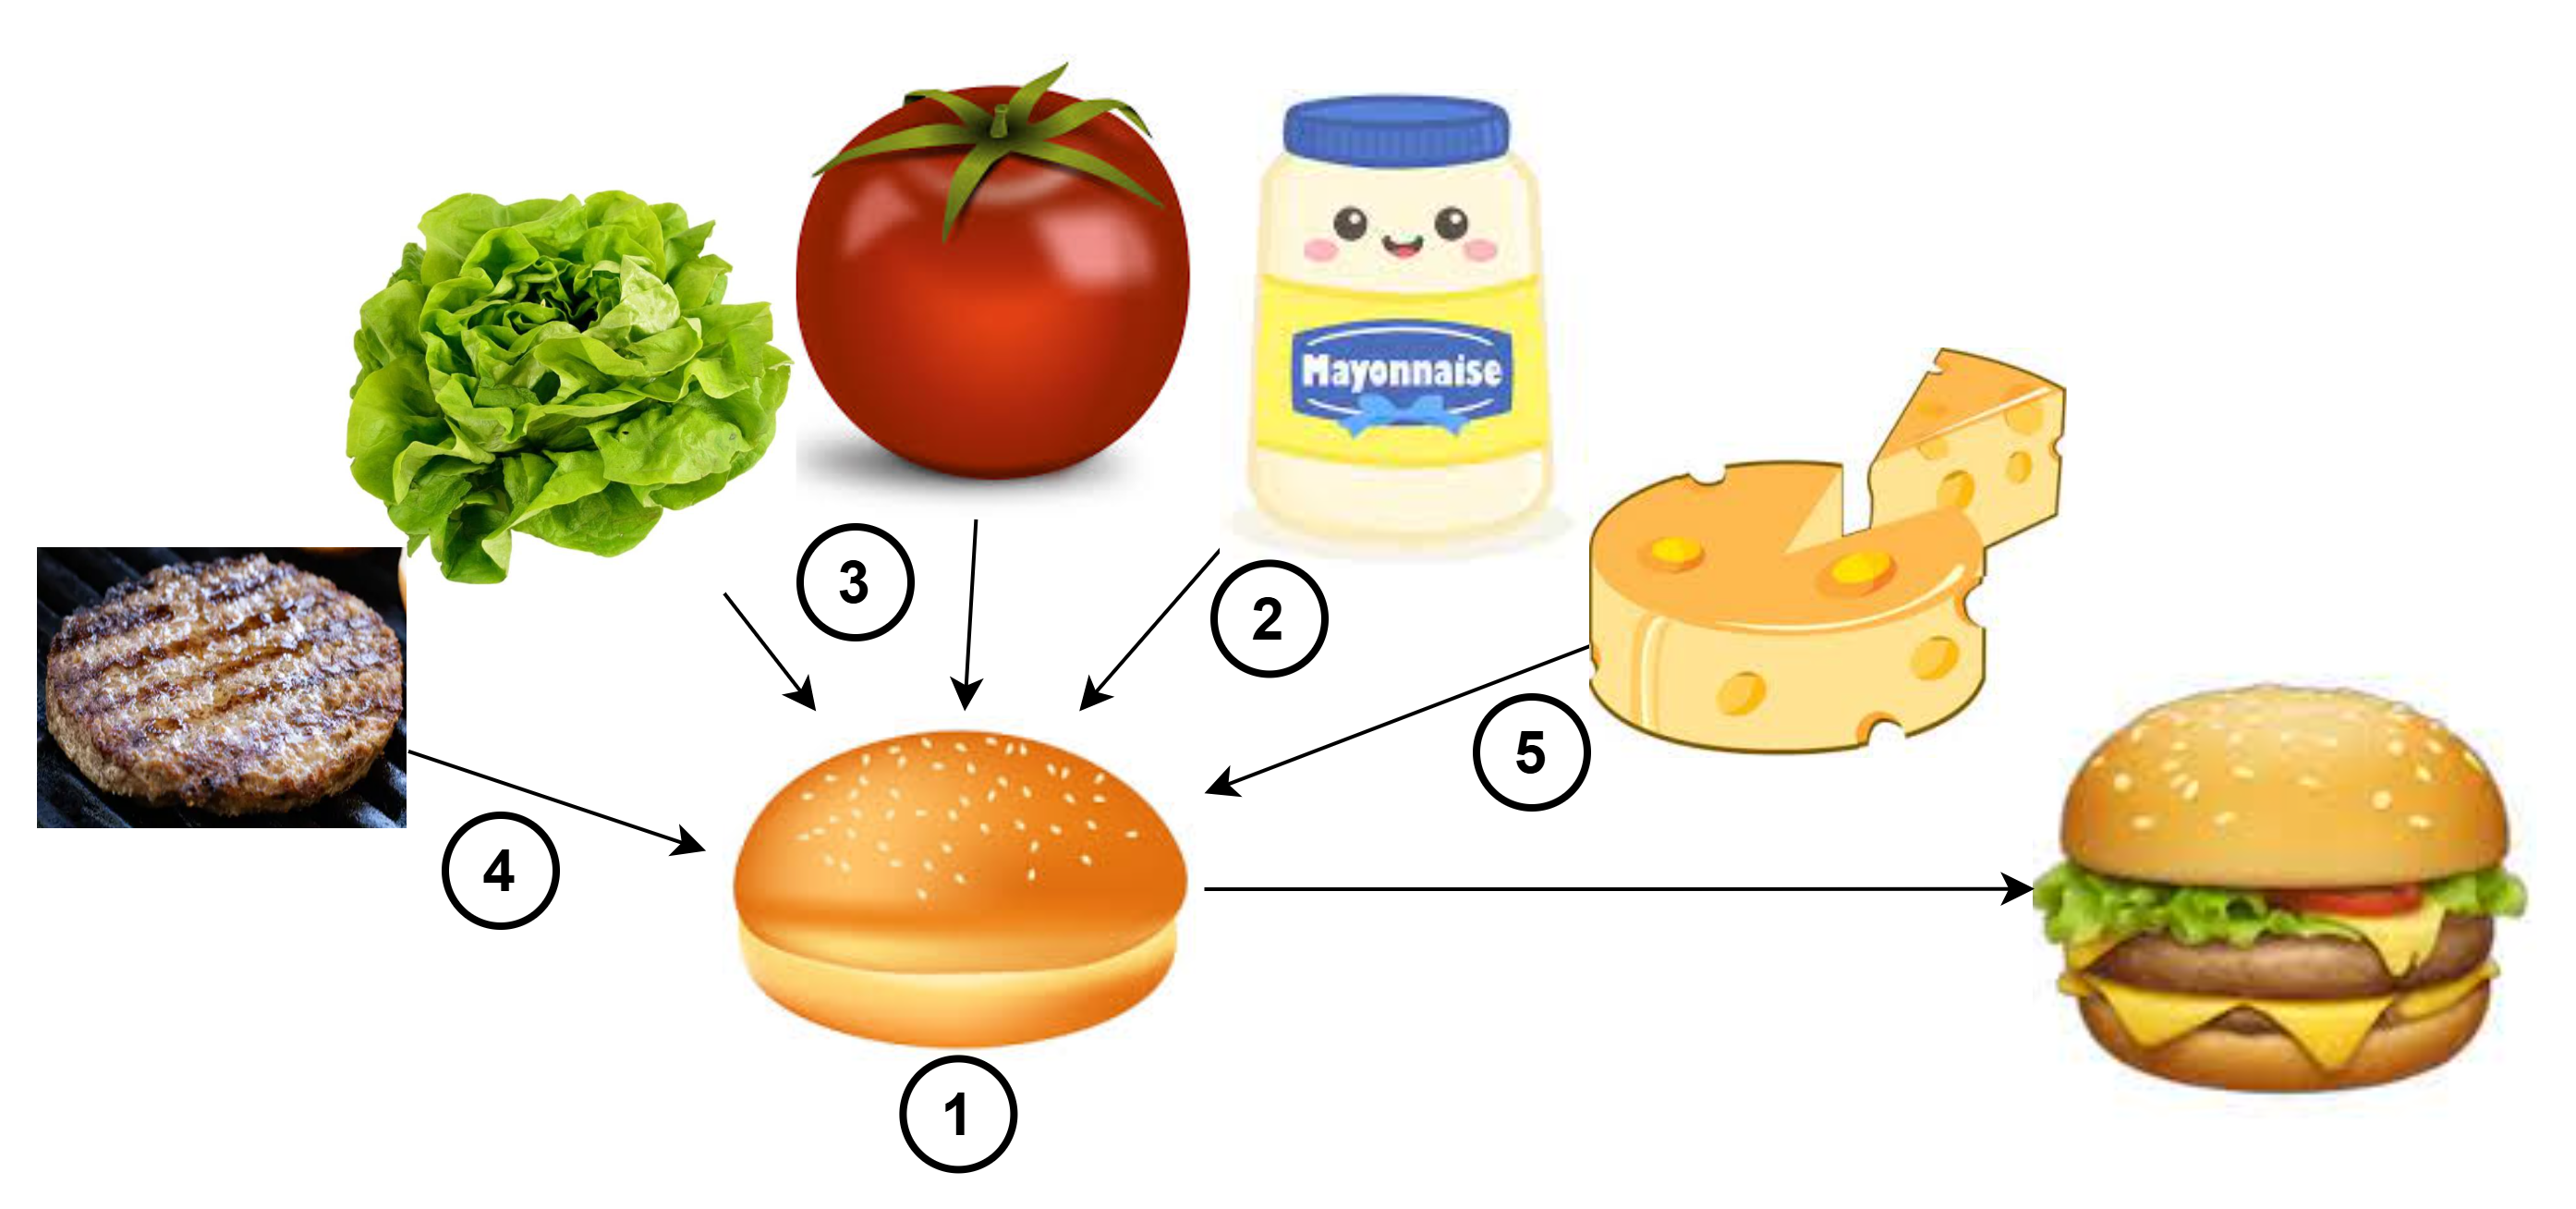
\includegraphics[width=0.9\textwidth]{../../figuras/algoritmo-hamburger-1.png}\\[-2ex]
		\caption{Diagrama do algoritmo 01.}
		\label{fig:Diagrama}
	\end{figure}
\end{frame}



\begin{frame}
	\frametitle{Fluxograma}
	Simbolos utilizados no fluxograma e seus significados:
	\begin{figure}
		\centering
		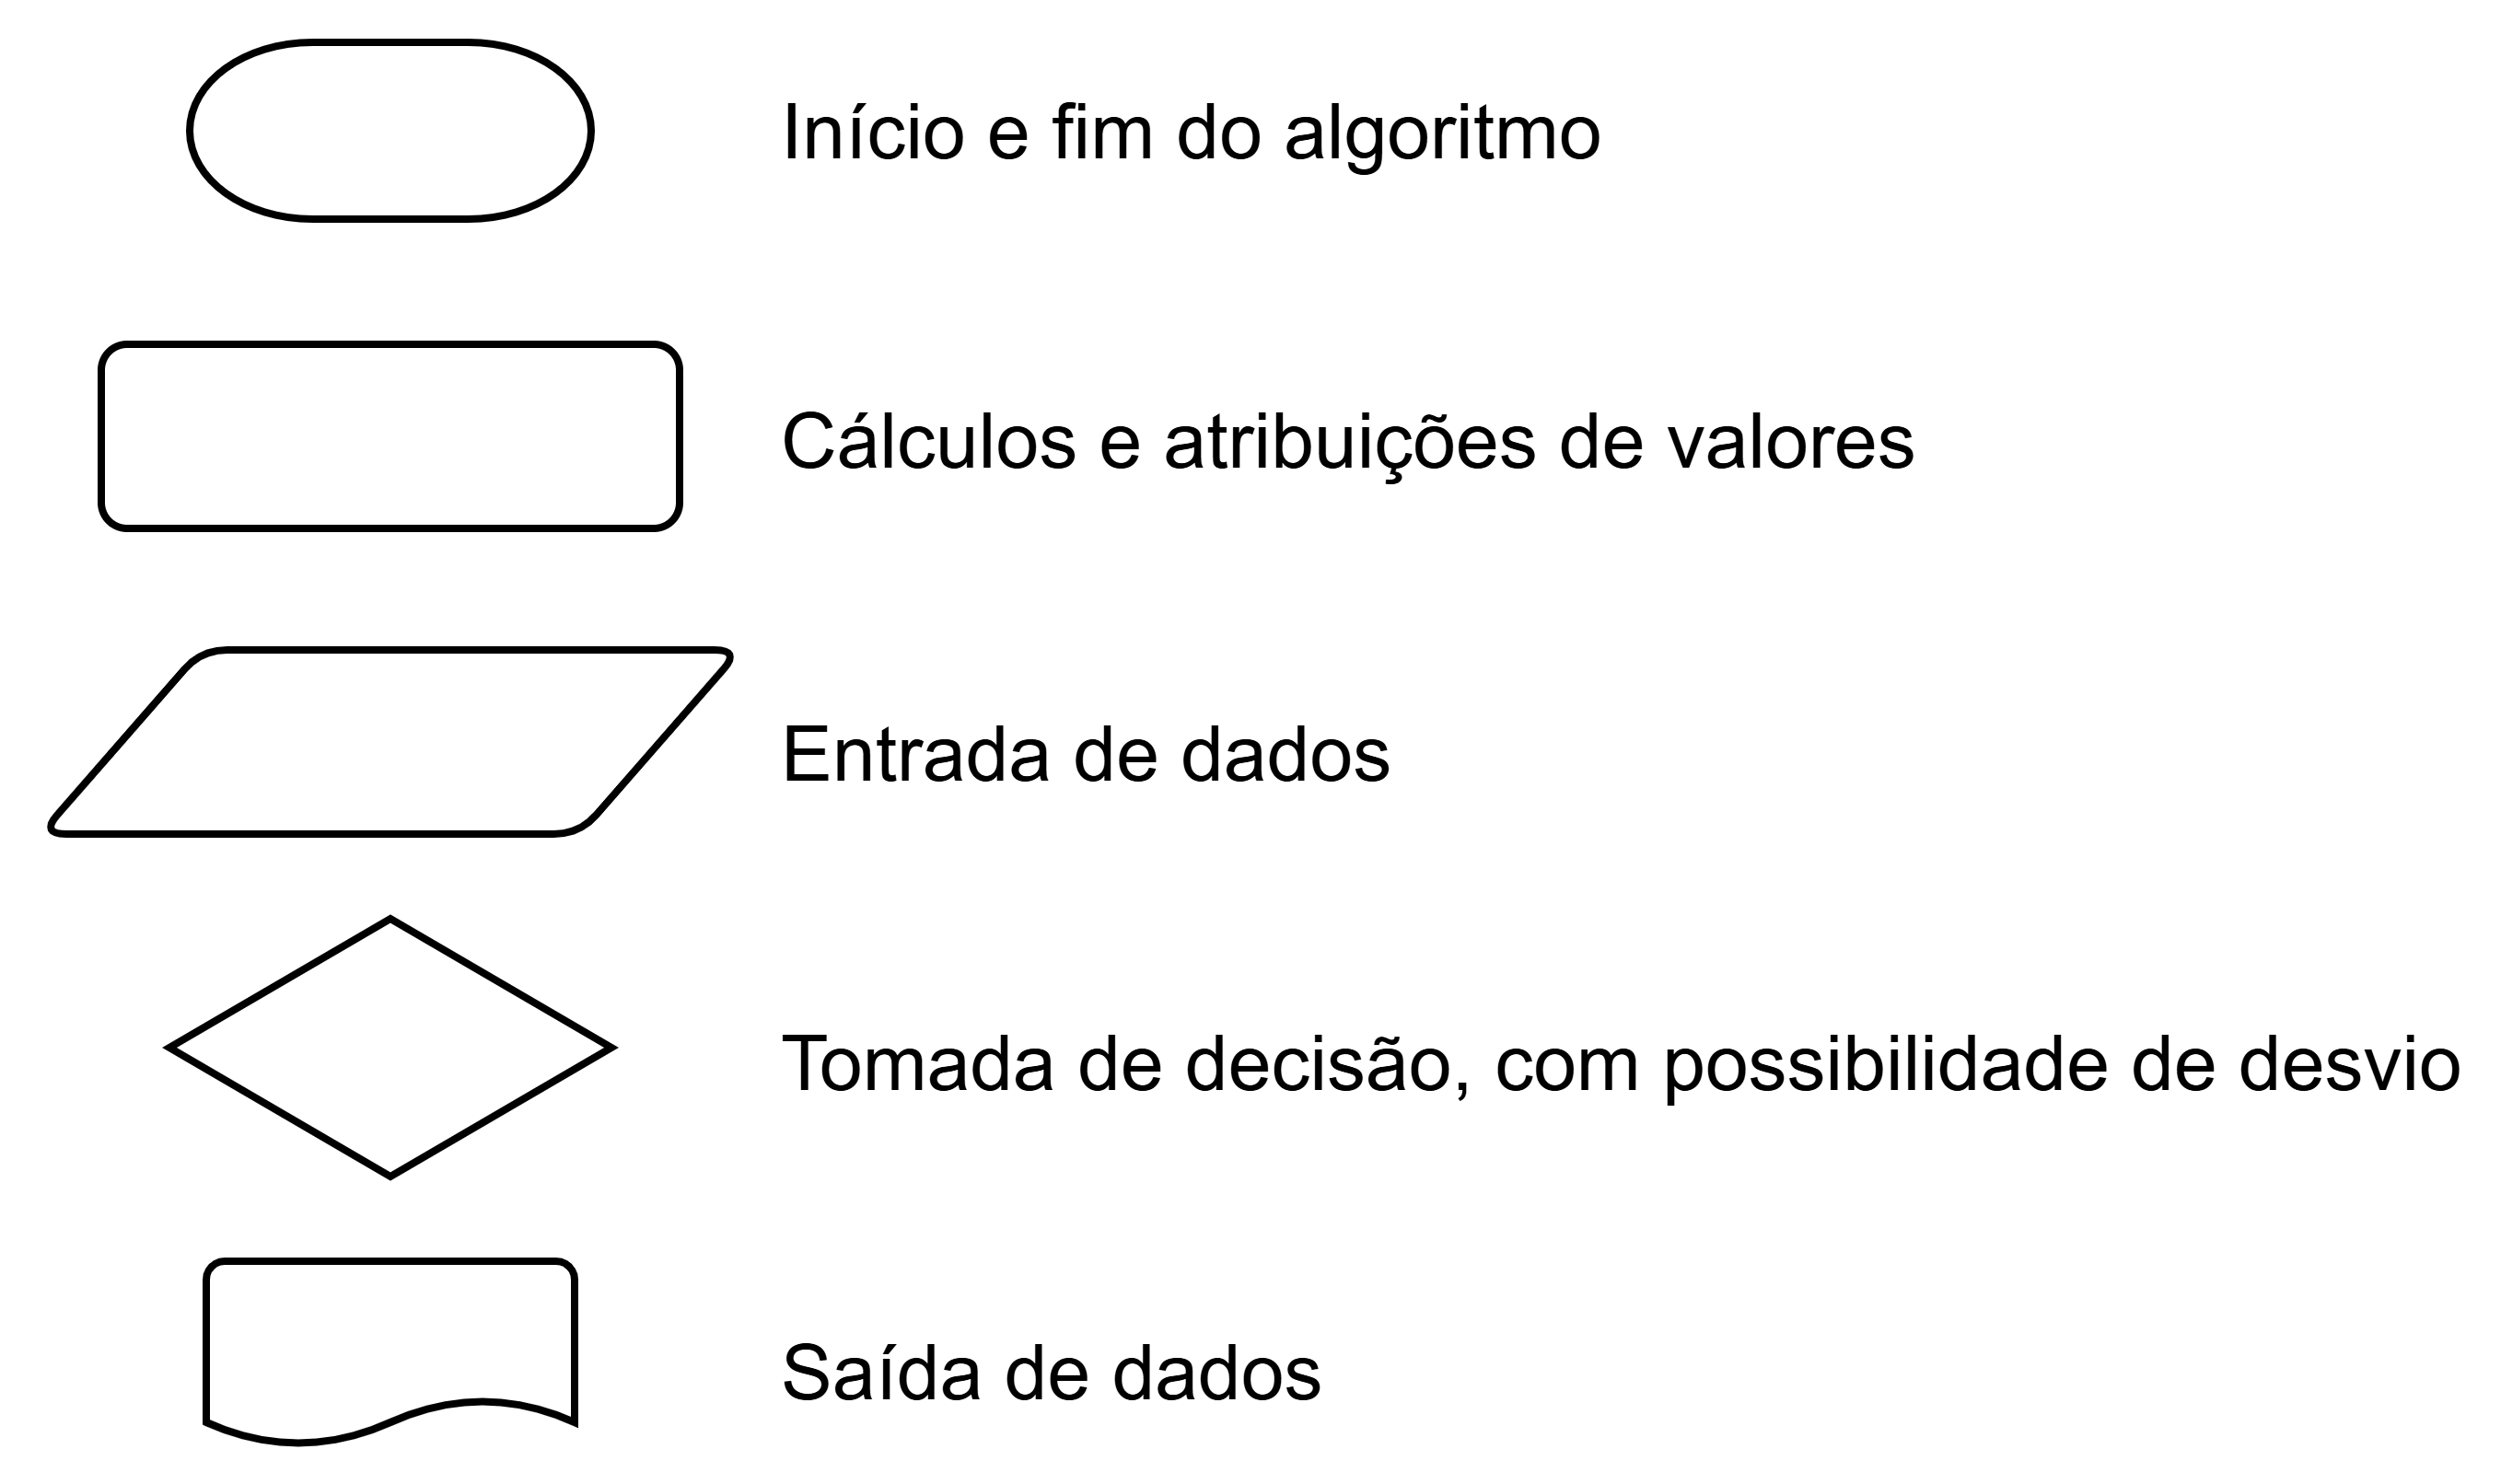
\includegraphics[width=0.8\textwidth]{../../figuras/simbolos-fluxograma.png}\\[-2ex]
		\caption{Símbolos para fluxograma de algoritmos.}
		\label{fig:Diagrama}
	\end{figure}
\end{frame}


\begin{frame}
	\frametitle{Fluxograma}
	Fluxograma do algoritmo para mostrar o resultado da multiplicação de dois números:
	\begin{figure}
		\centering
		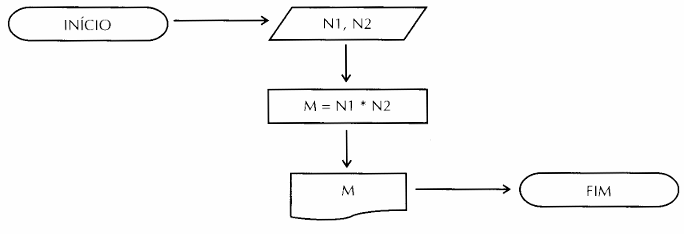
\includegraphics[width=0.8\textwidth]{../../figuras/exemplo-fluxograma.png}\\[-2ex]
		\caption{Exemplo de um Fluxograma.}
		\label{fig:exemplo-Fluxograma}
	\end{figure}
\end{frame}



\begin{frame}
	\frametitle{Técnicas para descrição de algoritmos}
	
	\begin{block}{\textbf{Pseudocódigo}}
		Escrever os passos por meio de texto com regras predefinidas ou estruturadas.
	\end{block}
	
	\textbf{Vantagem:} é bem próximo do código final.
	
	\textbf{Desvantagem:} tem que assimilar as regras que devem ser usadas.
	\textbf{Exemplo}: Somar dois números:

	\begin{block}{\textbf{Algoritmo em Pseudocódigo}}
		\texttt{ALGORITMO "somar dois números"}\\
		\texttt{INICIO}\\
		\texttt{DECLARE numero1, numero2, resultado NUMÉRICO}\\
		\texttt{ESCREVA "Digite dois número"}\\
		\texttt{LEIA numero1, numero2}\\
		\texttt{resultado $\leftarrow$ numero1 + numero2}\\
		\texttt{ESCREVA "A soma é = ", resultado}\\
		\texttt{FIMALGORITMO}
	\end{block}

\end{frame}





